\documentclass{mcmthesis}
\mcmsetup{CTeX = false,  
        tcn = 2302952, problem = D,
        sheet = true, titleinsheet = true, keywordsinsheet = true,
        titlepage = false, abstract = false}
\usepackage{newtxtext}
\title{Wisdom Hidden in Teaming Strategies}
\date{\today}
\begin{document}
\begin{abstract}
        For the first problem, we used Social Network Analysis to construct the passing network,
        and explained the basic attributes of the Network. Furthermore, specific network characteristics
        are analyzed from the perspective of whole network, local networks and individual networks.
        The whole network: the centroid. We also draw the timeline to
        analysis the dynamics of passing over time.

        Secondly, in order to measure team cooperation performance more comprehensively, this paper
        constructs a comprehensive evaluation index system by integrating Individual contributions to
        the team, Team structure, Strategic layout, Environment variables and 13 sub-indicators. Among
        them, in order to make clear the Individual contribution to the team, this paper combines
        subjective and objective weights, uses AHP and entropy weight to construct a sub-model of
        player scoring.

        Thirdly, after analyzing the structure that the Huskies often used in highlight
        performance., we find that the Huskies is more inclined to use defensive counterattack
        strategy. The Huskies usually performs better in the middle-front and back courts, but
        is very weak in the middle-back courts. Therefore, we recommend that the Huskies
        carries forward the long-pass punching mode.

        Finally, We further explore the possibility of applying
        the methods on general social activities.

        \begin{keywords}
                Teaming Strategies; Network Analysis; AHP and entropy weight;
        \end{keywords}
\end{abstract}
\maketitle
\tableofcontents
\newpage

\section{Introduction}
\subsection{Problem Background}
Nowadays, global demand for teamwork which are crucial for the development of the society has risen rapidly. As a competitive team sports, world football has ushered in a new hegemony without controversy. This let many football coach out of the cage to explore the methods of the winning game in the aspect of cooperation, especially in a typical team:Huskies. On the individual side, a star player may prompt the advantages of the teams into full play. However, despite the impacts of individual, the teamwork between teammates seem to be more significant to possess some good vibrations. Therefore, it is necessary to explore the rational teamwork strategies in a mathematically way and put forward some guides basing on the models for the Huskies coach.

\subsection{Problem Restatement}
\begin{itemize}
        \item Build a network which contains nodes and links for the ball passing to recognize the patterns and find out multiscales when observing the interaction.
        \item Determine the performance indicators reflected success and team level processes, and use them to construct a model to access the structure, configuration and dynamic of teamwork.
        \item Based on the teamwork model, tell the coach what structural strategies have been effective for the Huskies and what change can be made to promote success in the next competition.
        \item Discuss what other aspects of teamwork should be considered when generalizing the model of football teamwork to the team performance.
\end{itemize}

\section{Preparation of the Models}
\subsection{Assumptions}
\begin{itemize}
        \item The data provided is credible.
        \item Each player has equal strength.
        \item Anything not mentioned has no effect on the match, like weather, football field conditions and so on.
\end{itemize}
\subsection{Notations}
\begin{center}
        \begin{tabular}{cc}
                \toprule[1.5pt]
                \makebox[0.3\textwidth][c]{Symbol} & \makebox[0.4\textwidth][c]{Definition} \\
                \midrule[1pt]
                $w_{ij}$                           & adjacency matrix                       \\
                $c(i)$                             & node centrality                        \\
                $K_{i j}$                          & number of passes of two players        \\

                \bottomrule[1.5pt]
        \end{tabular}
\end{center}

\section{Passing Network Model Analysis}
\subsection{Network of First Match}
Considering the relationship between players on the football field, the network for
the ball passing can be described as an adjacency matrix in Data Structure. An adjacency
matrix can be generated to perform network analysis, which represents the
connections between a node (player) and an adjacency node (teammate). To generate
an adjacency matrix for network analysis, you must define criteria that characterize
the connections. We define $w_{ij}$ as the number of passes between player $i$ and player $j$.
The adjacency matrix between players can be expressed as:

\begin{equation}
        \begin{array}{l}
                \begin{array}{llll}
                         1 & 2 & \cdots \cdots \cdots & 11\\
                \end{array}                   \\
                \begin{array}{cccc}
                        1      \\
                        2      \\
                        \vdots \\
                        11
                \end{array}\left(\begin{array}{cccc}
                                                 w_{11}   & w_{12}   & \cdots & w_{1,11}  \\
                                                 w_{21}   & w_{21}   & \cdots & w_{2,11}  \\
                                                 \vdots   & \vdots   & \cdots & \vdots    \\
                                                 w_{11,1} & w_{11,2} & \cdots & w_{11,11}
                                         \end{array}\right) \\
        \end{array}
\end{equation}

\begin{figure}
        \centering
        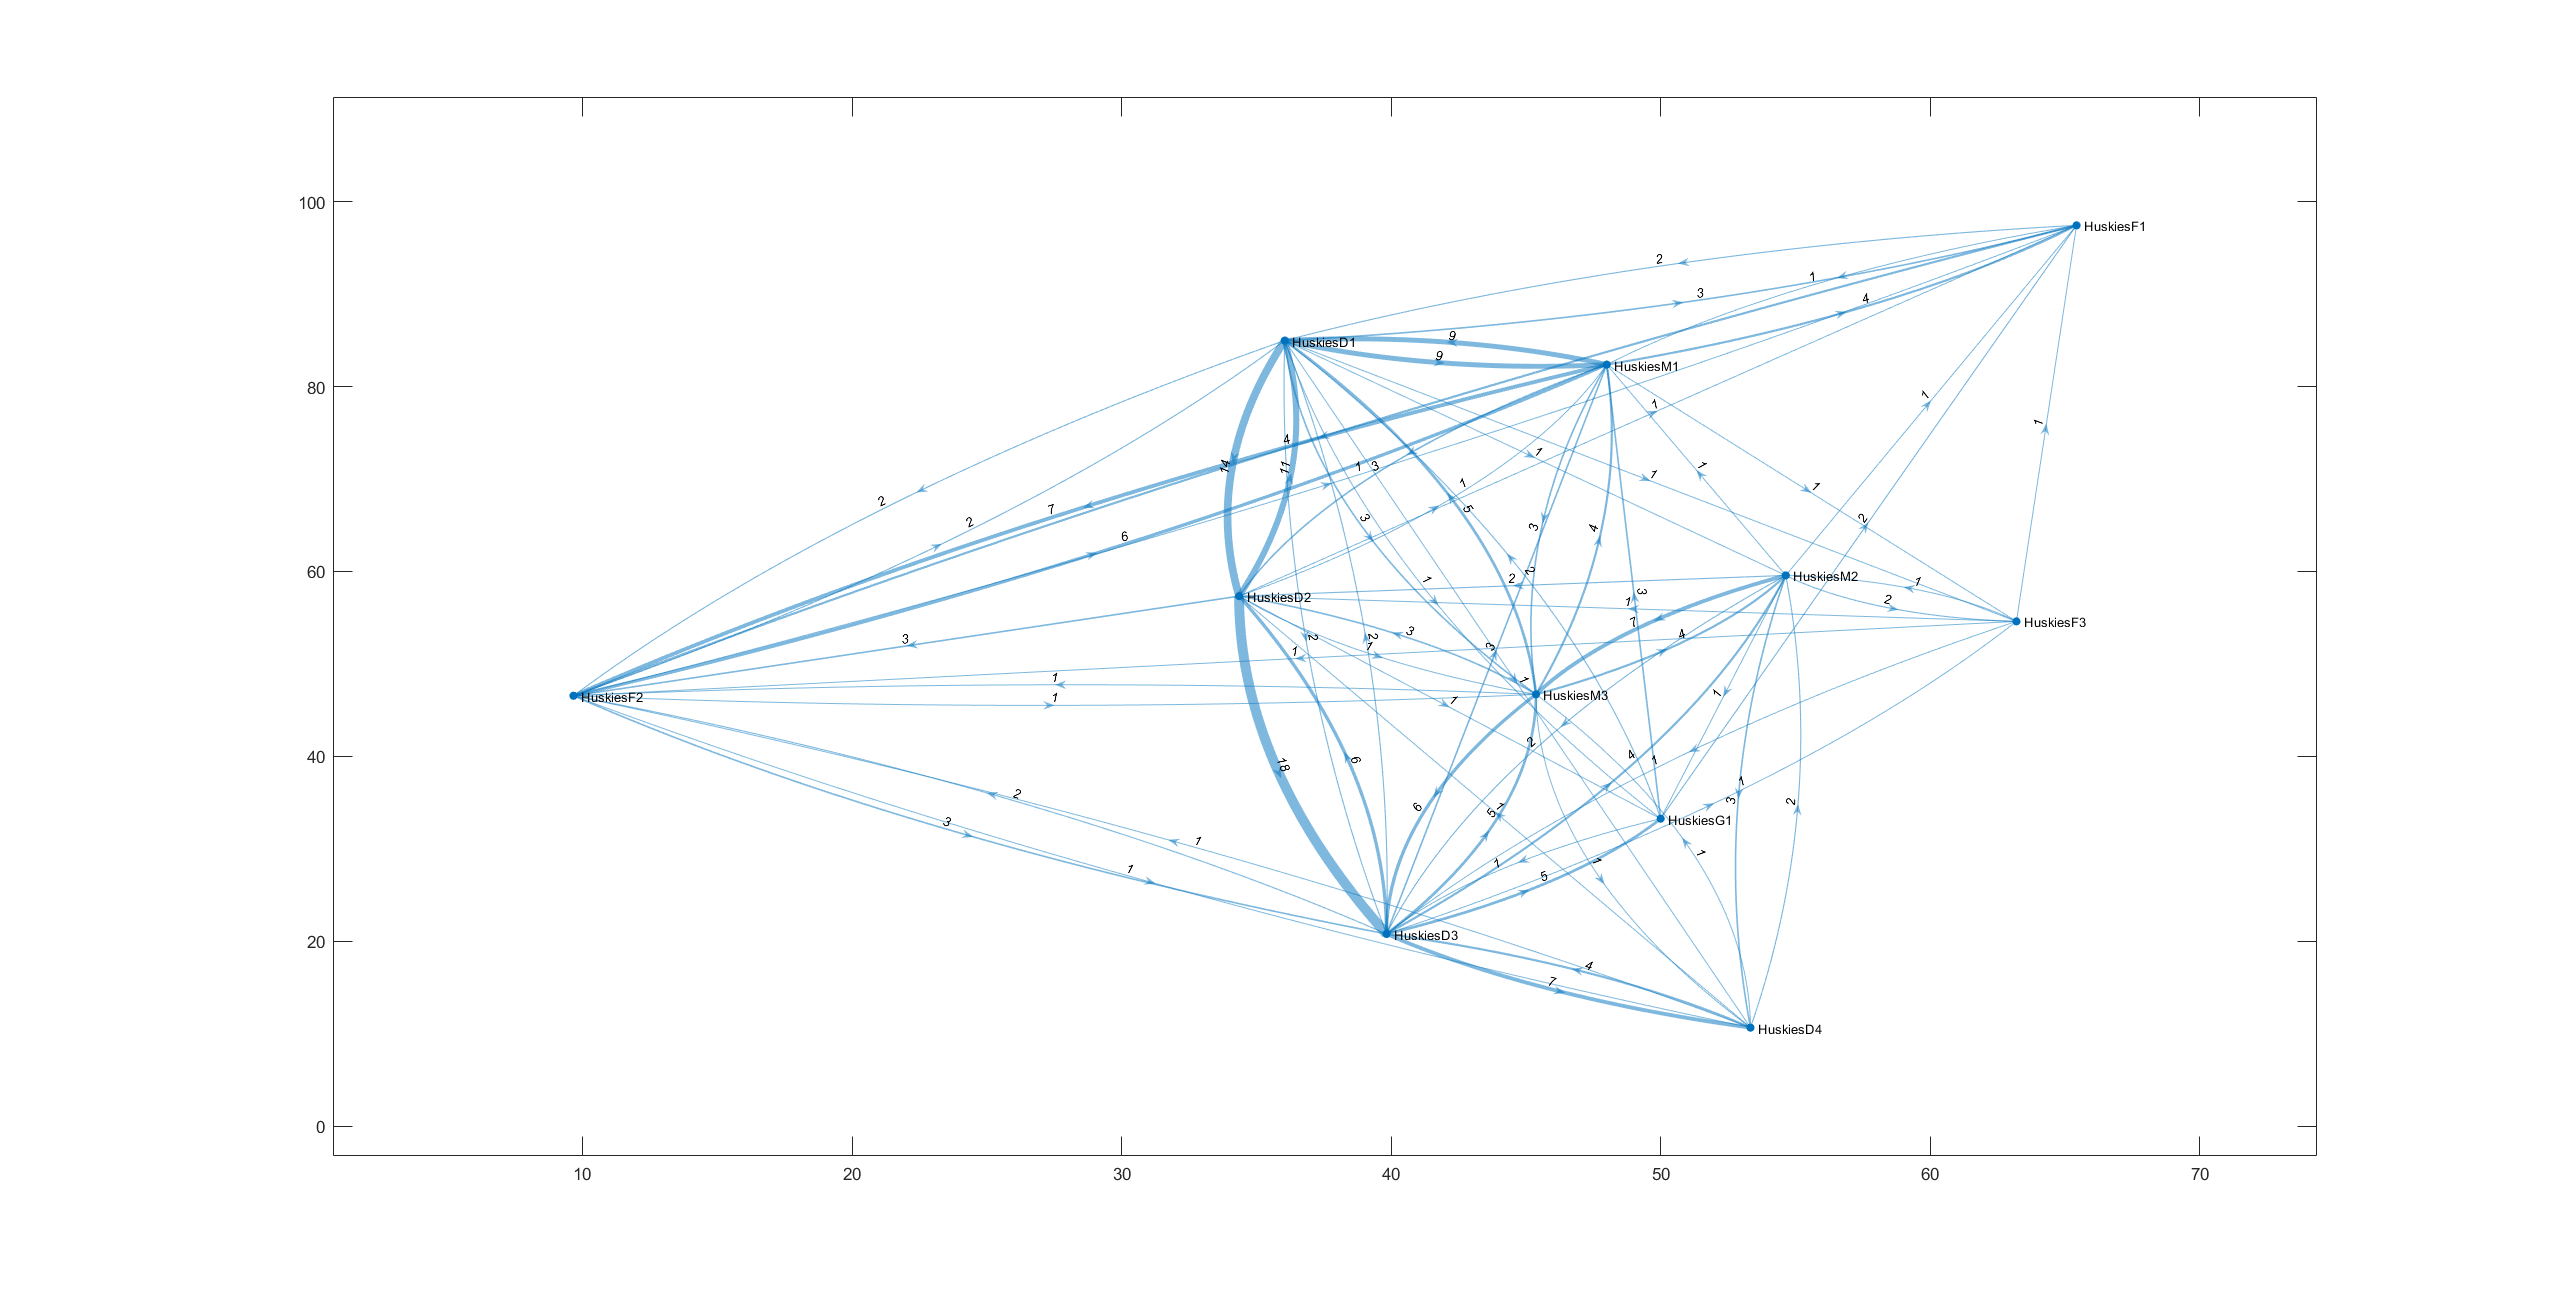
\includegraphics[height=0.3\textheight]{netH.png}
        \caption{Huskies' passing network of match 1(1H)}
\end{figure}

\begin{figure}
        \centering
        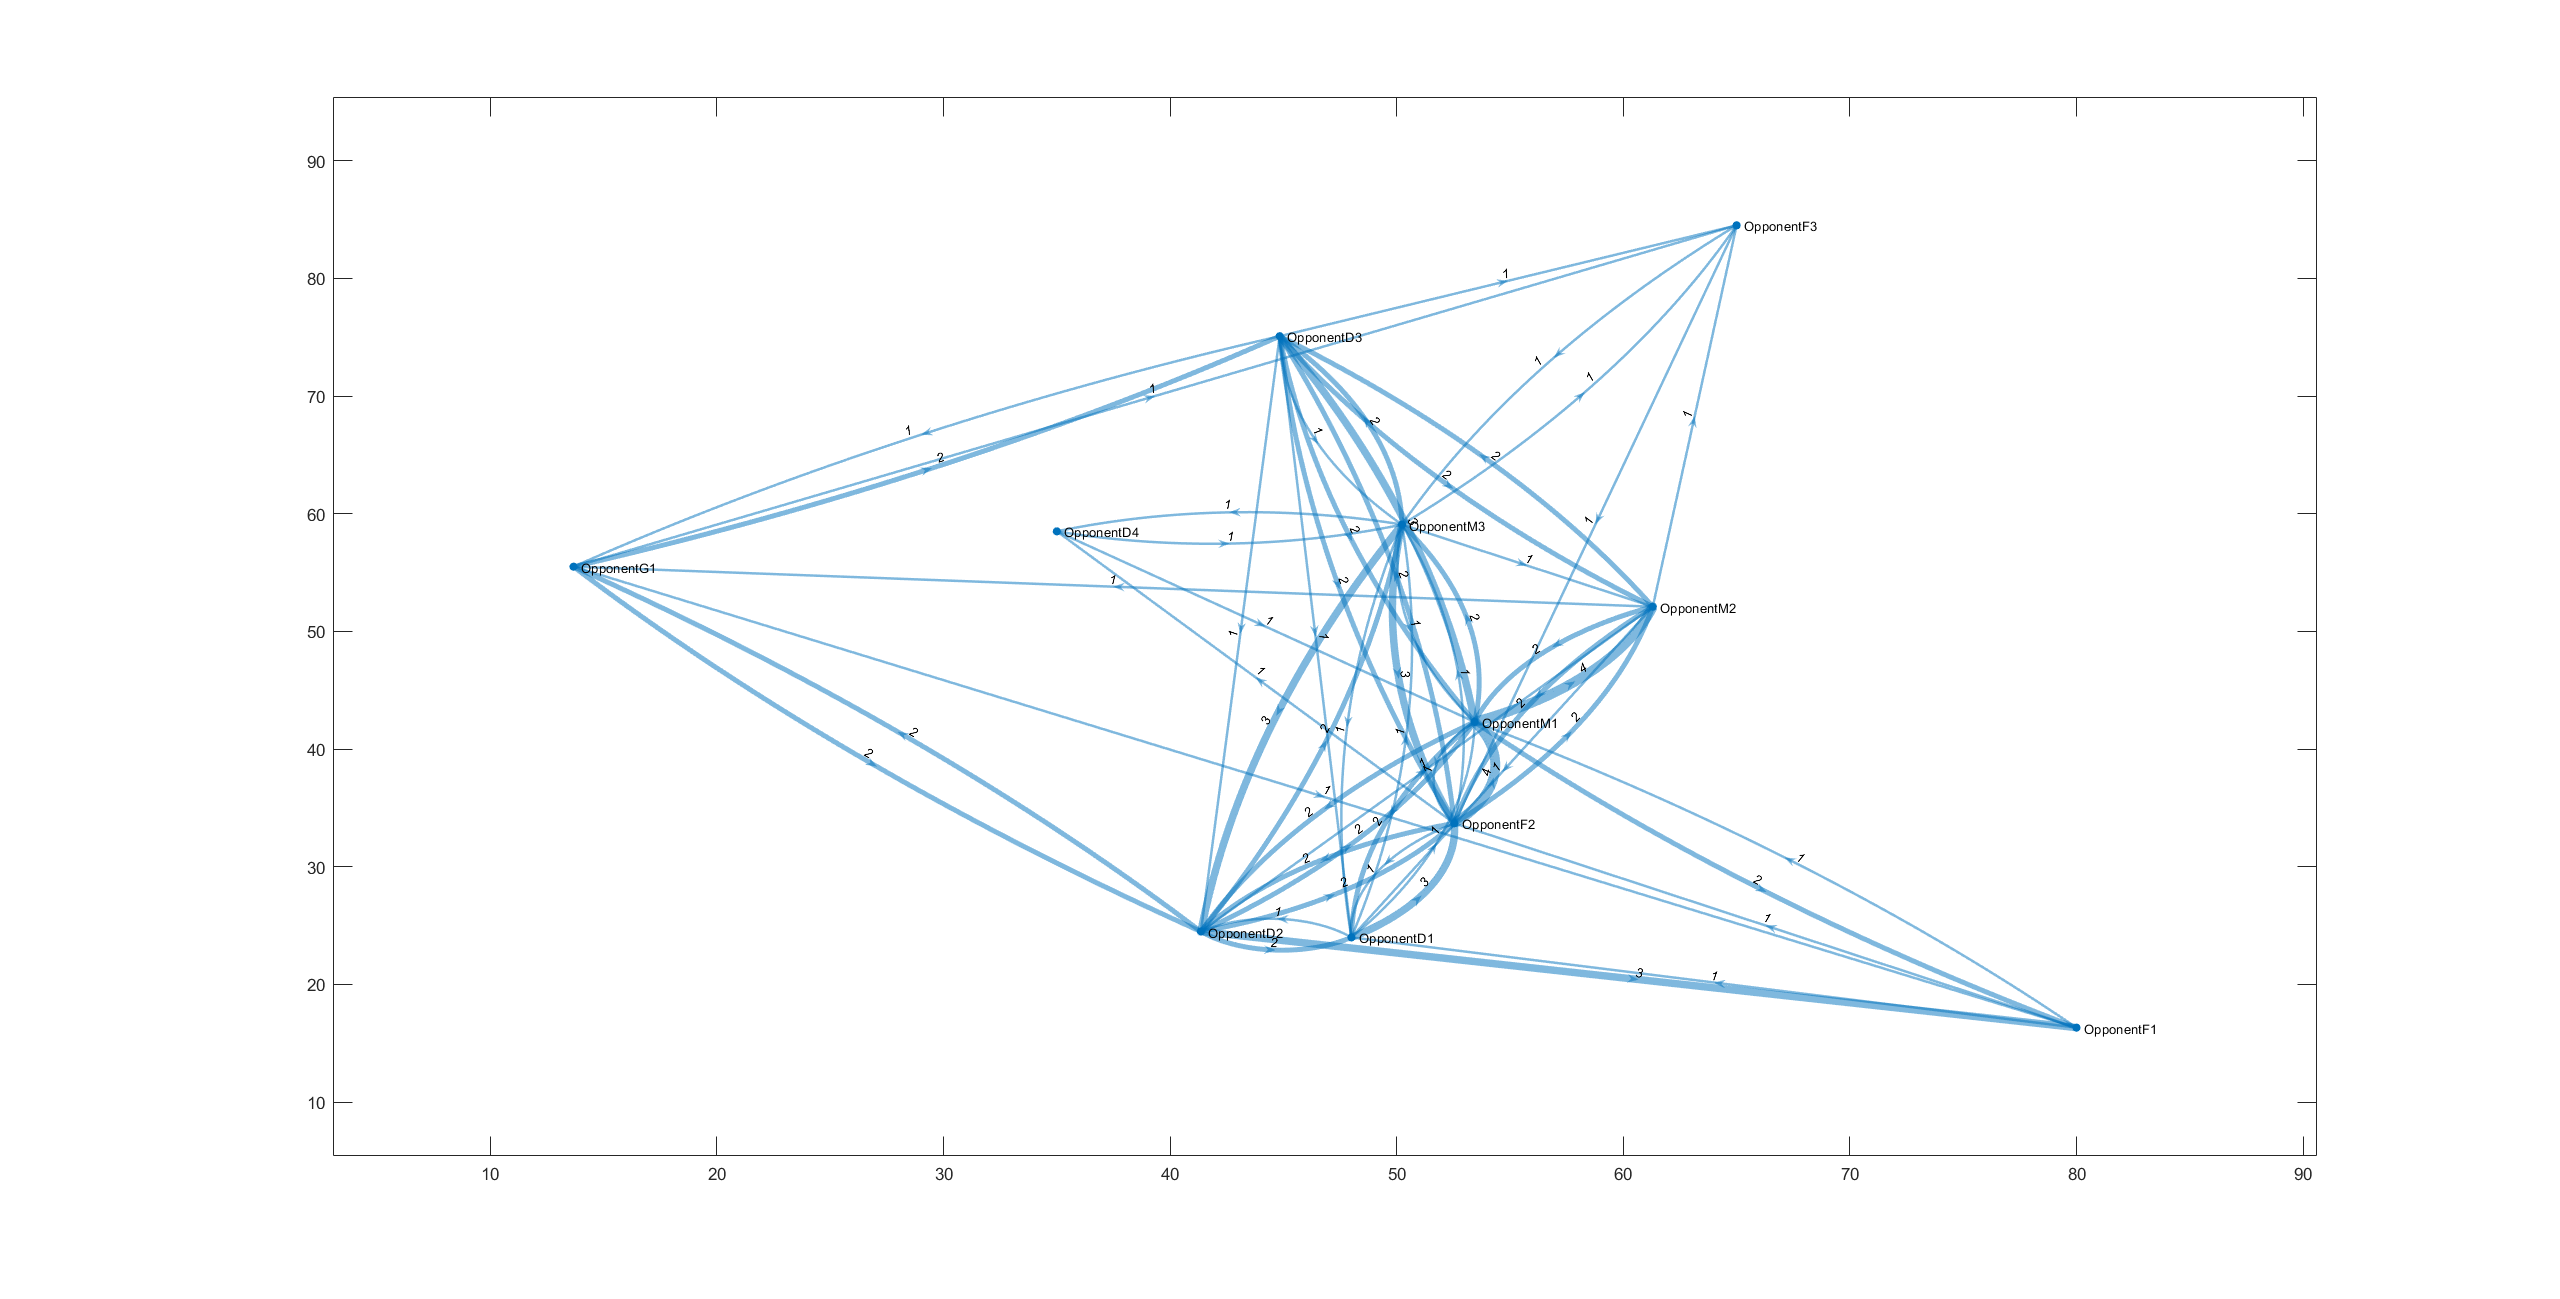
\includegraphics[height=0.3\textheight]{netO.png}
        \caption{Opponent's passing network of match 1(1H)}
\end{figure}

As shown in the figures above, the nodes in the network represent the players and the number of
nodes corresponds to the number of players on the field. The width of the
link indicates the weight, which is the number of passes contained in this link. The more times,
the wider the link. The position of each node depends on its average position, the average of
the coordinates of each player passing the ball, with the range of [0,100].

\subsection{Network patterns and properties}
\subsubsection{Node Centrality}
centrality types use the inverse sum of the distance from a node to all other nodes in the graph.
If not all nodes are reachable, then the centrality of node i is:

\begin{equation}
        c(i)=\left(\frac{A_{i}}{N-1}\right)^{2} \frac{1}{C_{i}}
\end{equation}

$A_i$ is the number of reachable nodes from node $i$ (not counting $i$), $N$ is the number of nodes in $G$, and $C_i$ is the sum of distances from node $i$ to all reachable nodes.

After calculation, Node Centrality can be added to the figures as follow.

\begin{figure}
        \centering
        \begin{minipage}[c]{0.45\textwidth}
                \centering
                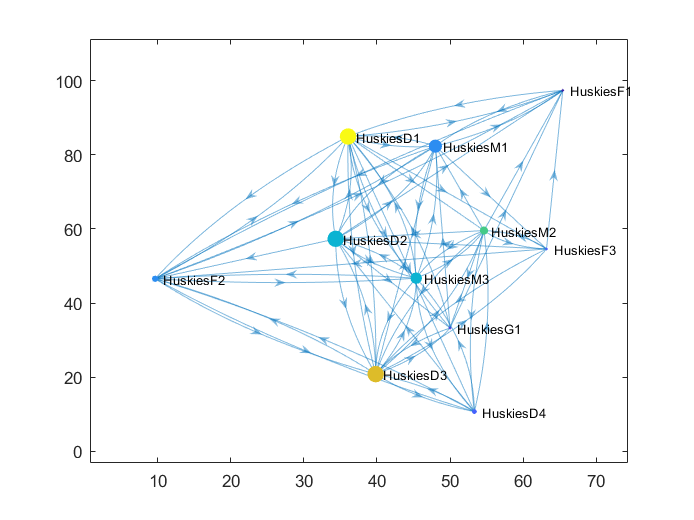
\includegraphics[height=0.2\textheight]{netAnalysis1.png}
        \end{minipage}
        \begin{minipage}[c]{0.45\textwidth}
                \centering
                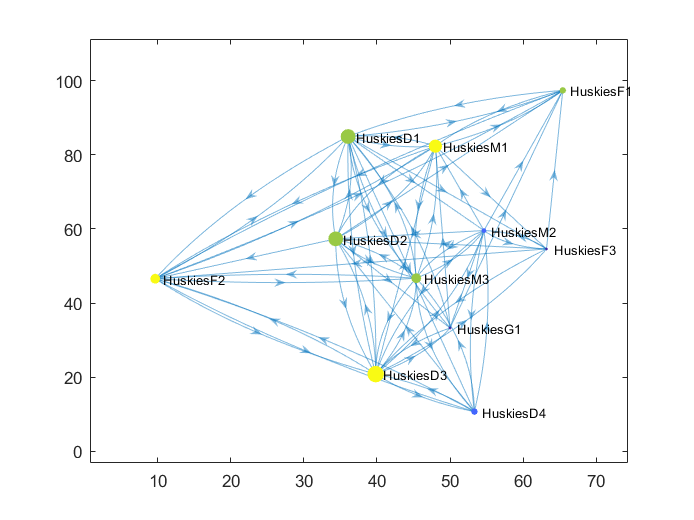
\includegraphics[height=0.2\textheight]{netAnalysis2.png}
        \end{minipage}
        \caption{Node Centrality of Huskies's match 1(1H)}
\end{figure}

According to the importance and degree of affinity of nodes, the nodes in the network are
divided into core nodes and edge nodes so as to simplify the complex network and focus on
the key structure of the network. Through the method of the core-periphery analysis, we can
get the core and periphery players of a team. The core player is generally a player as a critical
node that can connect the periphery player with the other core players. There will be more
passes between the core players and between the core players and the periphery players.
The results are that the team is formed by the core players 1, 2, 3, 4, 5, 6, 7, 10, 11 and 12,
and the periphery players 8, 9, 13 and 14. Combined with the positions of these players, link
thickness and the number of links connecting them, it can be found that the core players
above really play a role of interconnection and interaction.

\subsubsection{The timeline of passes in a match}
The timeline of passes can reflect the dynamic progress of the game, which is the change of
total passes in time. The Huskies' timeline is as follows:

\begin{figure}
        \centering
        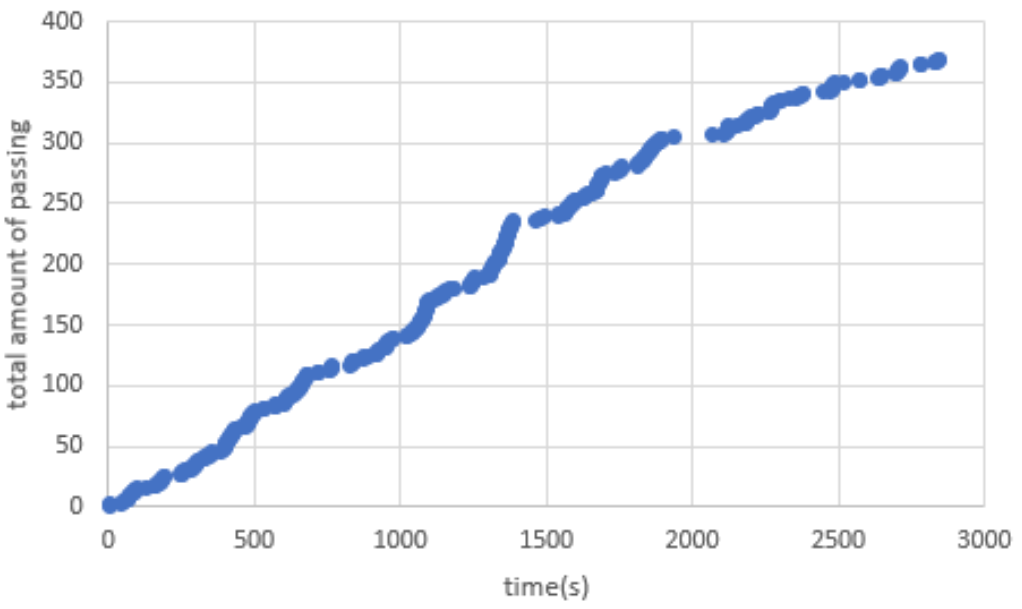
\includegraphics[height=0.3\textheight]{timeline.png}
        \caption{The frequency order and the most commonly used motif}
\end{figure}

The Huskies' passing volume increased evenly over all, with a flurry of passes occurring about
1,400 seconds after the game began.

\section{Teamwork Model}
\subsection{Individual contributions Model}
In a team, how much contribution each member has made to the team and the
distribution of individual contributions is one of the effective indicators to measure
team performance. In a team, players in different positions have different
responsibilities and division of labor. Therefore, it is illogical to evaluate each player's
contribution with a unified standard. In this section, we consider that players in
different positions will have different effects if they act with the same nature and will
form a new scoring standard by combining subjective and objective methods. We
combine analytic hierarchy process and entropy weight method to obtain different
weights of different positions and action types on the results, form scoring rules,
evaluate the contribution of each player, and then we can analyze the contribution
distribution of each team player in each match.

\subsubsection{Application of AHP in Establishment}
In this part, we use AHP to form a set of scoring rules. Analytic Hierarchy
Process (AHP) are in line with common sense, but there is a subjective problem in
index construction.

First, we construct the judgment matrix according to the rule of experience and
normalize it.

\begin{equation}
        K_{i j}=K_{i j} \div \sum_{i, j=1}^{n} K_{i j}
\end{equation}

Then we calculate the weight vector according to the normalized judgment
matrix and obtain the eigenvalues.

We use the consistency index CR to test, and CR<0.1 is found, so the
consistency test is passed.

\subsubsection{Application of Entropy Weight Method in Establishment}
The effect of each player's action on the result depends to a large extent on the
difference of the same type of action performed by players in the same position.
Based on this principle, entropy weight method can objectively evaluate the scoring
rules. The entropy weight method comprises the following steps:

As indicators are positive indicators, we
homogenize heterogeneous indicators according to the formula.

\begin{equation}
        y_{i j}=\frac{x_{i j}-\min \left(x_{. j}\right)}{\max \left(x_{. j}\right)-\min \left(x_{. j}\right)}
\end{equation}

Find the information entropy of each variable. For the $j^{th}$ variable, its
information entropy:

\begin{equation}
        \begin{array}{c}
                H_{j}=-\frac{1}{\ln n} \sum_{i=1}^{n} p_{i j} * \ln p_{i j} \\
                p_{i j}=\frac{y_{i j}}{\sum_{i=1}^{n} y_{i j}}
        \end{array}
\end{equation}

The information entropy of $J$ variables can be calculated above:$H_1,H_2, …,H_j$

\begin{equation}
        W_{j}=\frac{1-H_{j}}{P-\sum_{j=1}^{p} H_{j}}
\end{equation}

\section{Advice on Improving Team Success}
In this part we will analyze Huskies’ characteristics and offer some advice on structure.
The figure on the right side shows the difference between Huskies and other opponents on the
use of cooperation structure. The two green bars are above horizontal axis, showing the high
using frequency. Tactics three and five represents Midfield Overall Planning and Defensive
Shield respectively. Thus, we can infer that Huskies often use defensive counterattack strategy in
this season. In professional soccer pattern, this is called to be Long Ball. Players are waiting for
opportunities to break through opponents’ goal. When the time is ripe for an easy long ball,
forward can control the ball and shot.

After exploring Huskies’ common use cooperation structure, we need to find the most suitable
one. This figure shows the difference between Huskies and other opponents on the use of
cooperation structure during the highlight period.

\begin{figure}
        \centering
        \begin{minipage}[c]{0.45\textwidth}
                \centering
                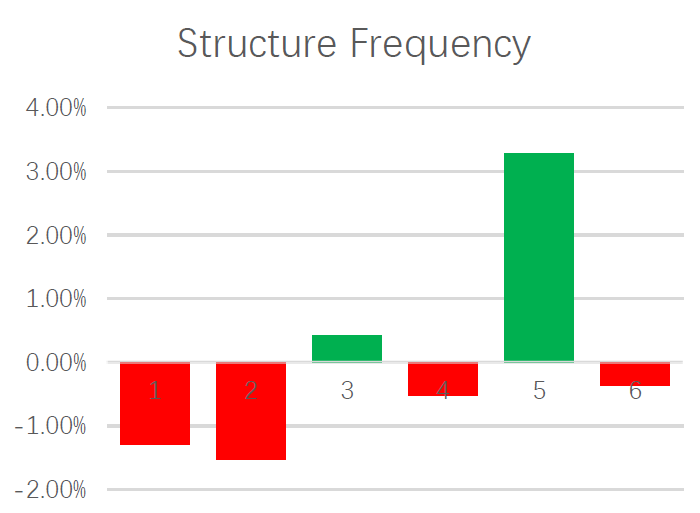
\includegraphics[height=0.2\textheight]{frequency.png}
        \end{minipage}
        \begin{minipage}[c]{0.45\textwidth}
                \centering
                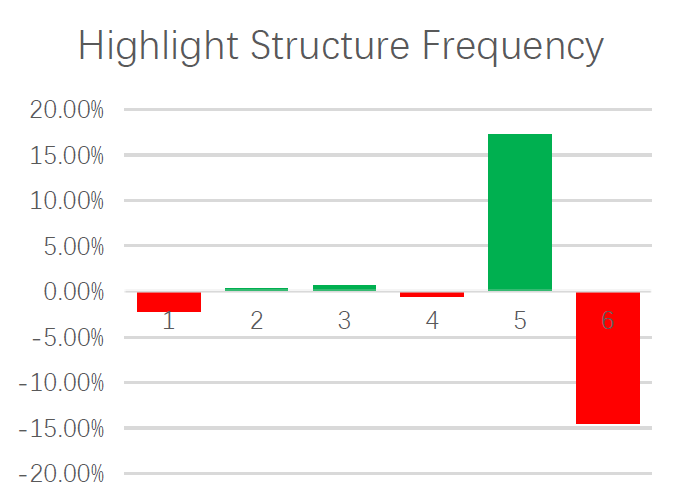
\includegraphics[height=0.2\textheight]{highlightFrequency.png}
        \end{minipage}
        \caption{Structure Frequency}
\end{figure}

This figure has obvious result and is more helpful to work out overall strategies. We can infer
that Huskies do well in structure two, three and five, which means Sidewalk Tiger, Defensive
Shield and Midfield Overall Planning respectively. When Huskies uses them, highlight
performance appears more easily.

Looking back on the figure below, we
discover that Huskies is more proficient
in backfield and mid-forth field while
really weak in mid-back field. Hence
Huskies is right to use counter attack and
long ball this season.

\subsection{Our Advice}
Reinforce to develop the skill of
counter attack and long ball in order
to produce the best possible results.
 From the Highlight Performance
figure, Sidewalk Tiger’s
performance is also slightly higher
than the average of whole season.
However, the using times of this
cooperation structure is smaller than
the average. Thus, we think it is
possible to make a break-through in
sidewalk attack.

\section{For Other Team Activities}
It is also possible to extend the method of network analysis to general social activities.
The key-point is to identify what is the key event in the problem, like pass events
in soccer games. For example, we want to investigate the relationships of researchers
in an area. We may construct a network based on how many papers two researchers
have co-authored. In this case, publishing a paper together is a key event. Suppose we
want to analyze the teamwork of employees in a company. We have many choices of
indicators to construct the network, depending on what are key events in this company.
Some key events can be attending a meeting together, emailing or making a phone call
to each other and so on.

\section{Strengths and weaknesses}
The advantages of this study lie in choosing models and indicators from a new
perspective and in combination with the characteristics of team cooperation of
football teams. The analysis level is clear, the results are stable, and the conclusions
and suggestions are practical. At the same time, there are still some unsolved
problems in this paper, such as limitations in the process of selecting indicators,
difficulty in quantifying the instantaneous positions of teammates and inability to
obtain the obstruction degree of opponents, etc. All of these require in-depth research
on the basis of expanding the number of indicators and sample size.

\newpage
\nocite{*}
\bibliographystyle{plain}
\bibliography{./reference/reference.bib}

\begin{appendices}
        \section{Code}
        \textbf{\textcolor[rgb]{0.98,0.00,0.00}{Input matlab source:}}
        \lstinputlisting[language=Matlab]{./code/Problem.m}
\end{appendices}
\end{document}
